%%%%%%%%%%%%%%%%%%%%%%%%%%%%%%%%%%%%%%%%%%%%%%%%%%%%%%%%%%%%%%%%%%%%%%%%%%%%%%%%
%Tutorial slides on Python.
%
% Author: FOSSEE 
% Copyright (c) 2009, FOSSEE, IIT Bombay
%%%%%%%%%%%%%%%%%%%%%%%%%%%%%%%%%%%%%%%%%%%%%%%%%%%%%%%%%%%%%%%%%%%%%%%%%%%%%%%%

\documentclass[14pt,compress]{beamer}
%\documentclass[draft]{beamer}
%\documentclass[compress,handout]{beamer}
%\usepackage{pgfpages} 
%\pgfpagesuselayout{2 on 1}[a4paper,border shrink=5mm]

% Modified from: generic-ornate-15min-45min.de.tex
\mode<presentation>
{
  \usetheme{Warsaw}
  \useoutertheme{infolines}
  \setbeamercovered{transparent}
}

\usepackage[english]{babel}
\usepackage[latin1]{inputenc}
%\usepackage{times}
\usepackage[T1]{fontenc}
\usepackage{amsmath}

% Taken from Fernando's slides.
\usepackage{ae,aecompl}
\usepackage{mathpazo,courier,euler}
\usepackage[scaled=.95]{helvet}

\definecolor{darkgreen}{rgb}{0,0.5,0}

\usepackage{listings}
\lstset{language=Python,
    basicstyle=\ttfamily\bfseries,
    commentstyle=\color{red}\itshape,
  stringstyle=\color{darkgreen},
  showstringspaces=false,
  keywordstyle=\color{blue}\bfseries}

%%%%%%%%%%%%%%%%%%%%%%%%%%%%%%%%%%%%%%%%%%%%%%%%%%%%%%%%%%%%%%%%%%%%%%
% Macros
\setbeamercolor{emphbar}{bg=blue!20, fg=black}
\newcommand{\emphbar}[1]
{\begin{beamercolorbox}[rounded=true]{emphbar} 
      {#1}
 \end{beamercolorbox}
}
\newcounter{time}
\setcounter{time}{0}
\newcommand{\inctime}[1]{\addtocounter{time}{#1}{\tiny \thetime\ m}}

\newcommand{\typ}[1]{\lstinline{#1}}

\newcommand{\kwrd}[1]{ \texttt{\textbf{\color{blue}{#1}}}  }

%%% This is from Fernando's setup.
% \usepackage{color}
% \definecolor{orange}{cmyk}{0,0.4,0.8,0.2}
% % Use and configure listings package for nicely formatted code
% \usepackage{listings}
% \lstset{
%    language=Python,
%    basicstyle=\small\ttfamily,
%    commentstyle=\ttfamily\color{blue},
%    stringstyle=\ttfamily\color{orange},
%    showstringspaces=false,
%    breaklines=true,
%    postbreak = \space\dots
% }


%%%%%%%%%%%%%%%%%%%%%%%%%%%%%%%%%%%%%%%%%%%%%%%%%%%%%%%%%%%%%%%%%%%%%%
% Title page
\title[Matrices \& Equations]{Python for Science and Engg: Matrices \& Solution of equations}

\author[FOSSEE] {FOSSEE}

\institute[IIT Bombay] {Department of Aerospace Engineering\\IIT Bombay}
\date[] {31, October 2009\\Day 1, Session 4}
%%%%%%%%%%%%%%%%%%%%%%%%%%%%%%%%%%%%%%%%%%%%%%%%%%%%%%%%%%%%%%%%%%%%%%

%\pgfdeclareimage[height=0.75cm]{iitmlogo}{iitmlogo}
%\logo{\pgfuseimage{iitmlogo}}


%% Delete this, if you do not want the table of contents to pop up at
%% the beginning of each subsection:
\AtBeginSubsection[]
{
  \begin{frame}<beamer>
    \frametitle{Outline}
    \tableofcontents[currentsection,currentsubsection]
  \end{frame}
}

\AtBeginSection[]
{
  \begin{frame}<beamer>
    \frametitle{Outline}
    \tableofcontents[currentsection,currentsubsection]
  \end{frame}
}

% If you wish to uncover everything in a step-wise fashion, uncomment
% the following command: 
%\beamerdefaultoverlayspecification{<+->}

%\includeonlyframes{current,current1,current2,current3,current4,current5,current6}

%%%%%%%%%%%%%%%%%%%%%%%%%%%%%%%%%%%%%%%%%%%%%%%%%%%%%%%%%%%%%%%%%%%%%%
% DOCUMENT STARTS
\begin{document}

\begin{frame}
  \titlepage
\end{frame}

\begin{frame}
  \frametitle{Outline}
  \tableofcontents
%  \pausesections
\end{frame}

\section{Matrices}

\begin{frame}
\frametitle{Matrices: Introduction}
Let us now look at matrices in detail.\\
\alert{All matrix operations are done using \kwrd{arrays}}
\end{frame}

\subsection{Initializing}
\begin{frame}[fragile]
\frametitle{Matrices: Initializing}
\begin{lstlisting}
In []: A = array([[ 1,  1,  2, -1],
                  [ 2,  5, -1, -9],
                  [ 2,  1, -1,  3],
                  [ 1, -3,  2,  7]])
In []: A
Out[]: 
array([[ 1,  1,  2, -1],
       [ 2,  5, -1, -9],
       [ 2,  1, -1,  3],
       [ 1, -3,  2,  7]])
\end{lstlisting}
\end{frame}

\begin{frame}[fragile]
  \frametitle{Accessing elements of matrices}
\begin{small}
  \begin{lstlisting}
In []: C = array([[1,1,2],
                  [2,4,1],
                  [-1,3,7]])
In []: C[1,2]
Out[]: 1

In []: C[1]
Out[]: array([2, 4, 1])

In []: C[1,1] = -2
In []: C
Out[]: 
array([[ 1,  1,  2],
       [ 2, -2,  1],
       [-1,  3,  7]])
  \end{lstlisting}
\end{small}
\end{frame}

\subsection{Basic Operations}

\begin{frame}[fragile]
\frametitle{Transpose of a Matrix}
\begin{lstlisting}
In []: A.T
Out[]:
array([[ 1,  2,  2,  1],
       [ 1,  5,  1, -3],
       [ 2, -1, -1,  2],
       [-1, -9,  3,  7]])
\end{lstlisting}
\end{frame}

\begin{frame}[fragile]
  \frametitle{Sum of all elements}
  \begin{lstlisting}
In []: sum(A)
Out[]: 12
  \end{lstlisting}
\end{frame}

\begin{frame}[fragile]
  \frametitle{Matrix Addition}
  \begin{lstlisting}
In []: B = array([[3,2,-1,5],
                  [2,-2,4,9],
                  [-1,0.5,-1,-7],
                  [9,-5,7,3]])
In []: A + B
Out[]: 
array([[  4. ,   3. ,   1. ,   4. ],
       [  4. ,   3. ,   3. ,   0. ],
       [  1. ,   1.5,  -2. ,  -4. ],
       [ 10. ,  -8. ,   9. ,  10. ]])
  \end{lstlisting}
\end{frame}

\begin{frame}[fragile]
\frametitle{Elementwise Multiplication}
\begin{lstlisting}
In []: A*B
Out[]: 
array([[  3. ,   2. ,  -2. ,  -5. ],
       [  4. , -10. ,  -4. , -81. ],
       [ -2. ,   0.5,   1. , -21. ],
       [  9. ,  15. ,  14. ,  21. ]])

\end{lstlisting}
\end{frame}

\begin{frame}[fragile]
\frametitle{Matrix Multiplication}
\begin{lstlisting}
In []: dot(A,B)
Out[]: 
array([[ -6. ,   6. ,  -6. ,  -3. ],
       [-64. ,  38.5, -44. ,  35. ],
       [ 36. , -13.5,  24. ,  35. ],
       [ 58. , -26. ,  34. , -15. ]])
\end{lstlisting}
\end{frame}

\begin{frame}[fragile]
\frametitle{Inverse of a Matrix}
\begin{lstlisting}
In []: inv(A)
\end{lstlisting}
\begin{small}
\begin{lstlisting}
Out[]: 
array([[-0.5 ,  0.55, -0.15,  0.7 ],
       [ 0.75, -0.5 ,  0.5 , -0.75],
       [ 0.5 , -0.15, -0.05, -0.1 ],
       [ 0.25, -0.25,  0.25, -0.25]])
\end{lstlisting}
\end{small}
\end{frame}

\begin{frame}[fragile]
\frametitle{Determinant}
\begin{lstlisting}
In []: det(A)
Out[]: 80.0
\end{lstlisting}
\end{frame}

%%use S=array(X,Y)
\begin{frame}[fragile]
\frametitle{Eigenvalues and Eigen Vectors}
\begin{small}
\begin{lstlisting}
In []: E = array([[3,2,4],[2,0,2],[4,2,3]])

In []: eig(E)
Out[]: 
(array([-1.,  8., -1.]),
 array([[-0.74535599,  0.66666667, -0.1931126 ],
        [ 0.2981424 ,  0.33333333, -0.78664085],
        [ 0.59628479,  0.66666667,  0.58643303]]))

In []: eigvals(E)
Out[]: array([-1.,  8., -1.])
\end{lstlisting}
\end{small}
\end{frame}

\begin{frame}[fragile]
\frametitle{Computing Norms}
\begin{lstlisting}
In []: norm(E)
Out[]: 8.1240384046359608
\end{lstlisting}
\end{frame}

\begin{frame}[fragile]
  \frametitle{Singular Value Decomposition}
  \begin{small}
  \begin{lstlisting}
In []: svd(E)
Out[]: 
(array(
[[ -6.66666667e-01,  -1.23702565e-16,   7.45355992e-01],
 [ -3.33333333e-01,  -8.94427191e-01,  -2.98142397e-01],
 [ -6.66666667e-01,   4.47213595e-01,  -5.96284794e-01]]),
 array([ 8.,  1.,  1.]),
 array([[-0.66666667, -0.33333333, -0.66666667],
        [-0.        ,  0.89442719, -0.4472136 ],
        [-0.74535599,  0.2981424 ,  0.59628479]]))
  \end{lstlisting}
  \end{small}
\inctime{15}
\end{frame}

\section{Least Squares Fit}
\begin{frame}[fragile]
\frametitle{Least Squares Fit}
\vspace{-0.15in}
\begin{figure}
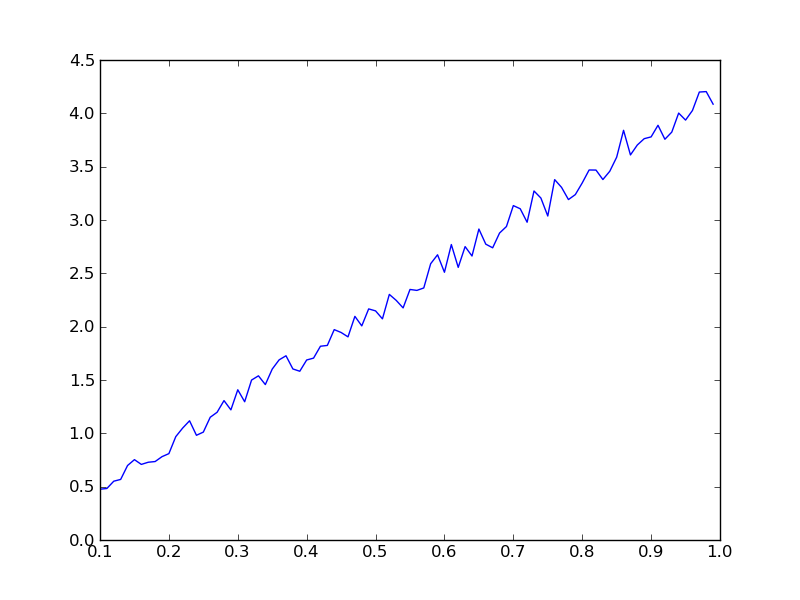
\includegraphics[width=4in]{data/L-Tsq-Line.png}
\end{figure}
\end{frame}

\begin{frame}[fragile]
\frametitle{Least Squares Fit}
\vspace{-0.15in}
\begin{figure}
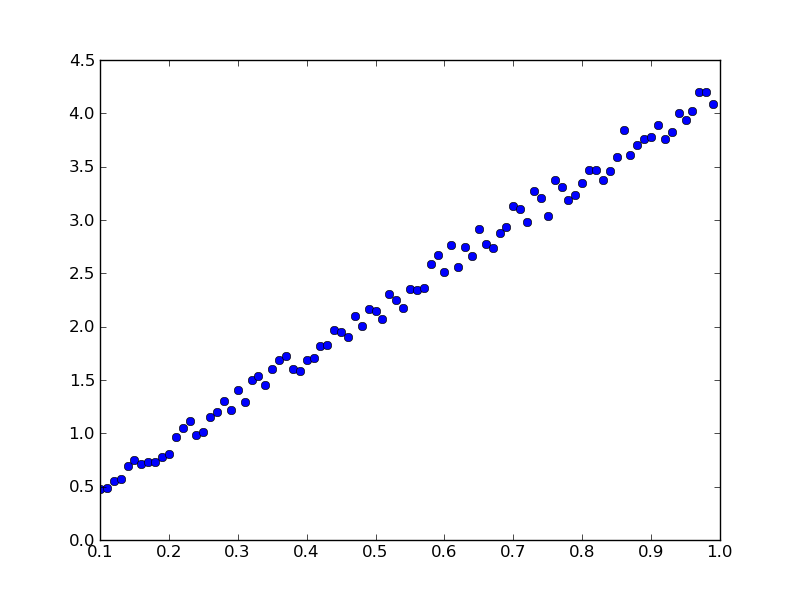
\includegraphics[width=4in]{data/L-Tsq-points.png}
\end{figure}
\end{frame}

\begin{frame}[fragile]
\frametitle{Least Squares Fit}
\vspace{-0.15in}
\begin{figure}
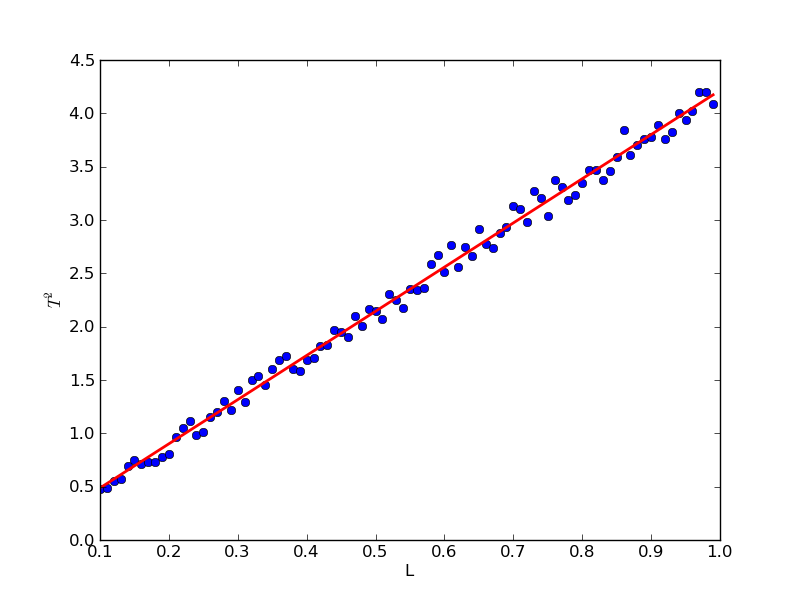
\includegraphics[width=4in]{data/least-sq-fit.png}
\end{figure}
\end{frame}

\begin{frame}
\frametitle{Least Square Fit Curve}
\begin{itemize}
\item $T^2$ and $L$ have a linear relationship
\item Hence, Least Square Fit Curve is a line
\item we shall use the \typ{lstsq} function
\end{itemize}
\end{frame}

\begin{frame}[fragile]
\frametitle{\typ{lstsq}}
\begin{itemize}
\item We need to fit a line through points for the equation $T^2 = m \cdot L+c$
\item The equation can be re-written as $T^2 = A \cdot p$
\item where A is   
  $\begin{bmatrix}
  L_1 & 1 \\
  L_2 & 1 \\
  \vdots & \vdots\\
  L_N & 1 \\
  \end{bmatrix}$
  and p is 
  $\begin{bmatrix}
  m\\
  c\\
  \end{bmatrix}$
\item We need to find $p$ to plot the line
\end{itemize}
\end{frame}

\begin{frame}[fragile]
\frametitle{Generating $A$}
\begin{lstlisting}
In []: A = array([L, ones_like(L)])
In []: A = A.T
\end{lstlisting}
%% \begin{itemize}
%% \item A is also called a Van der Monde matrix
%% \item It can also be generated using \typ{vander}
%% \end{itemize}
%% \begin{lstlisting}
%% In []: A = vander(L, 2)
%% \end{lstlisting}
\end{frame}

\begin{frame}[fragile]
\frametitle{\typ{lstsq} \ldots}
\begin{itemize}
\item Now use the \typ{lstsq} function
\item Along with a lot of things, it returns the least squares solution
\end{itemize}
\begin{lstlisting}
In []: coef, res, r, s = lstsq(A,TSq)
\end{lstlisting}
\end{frame}

\subsection{Plotting}
\begin{frame}[fragile]
\frametitle{Least Square Fit Line \ldots}
We get the points of the line from \typ{coef}
\begin{lstlisting}
In []: Tline = coef[0]*L + coef[1]
\end{lstlisting}
\begin{itemize}
\item Now plot Tline vs. L, to get the Least squares fit line. 
\end{itemize}
\begin{lstlisting}
In []: plot(L, Tline)
\end{lstlisting}
\end{frame}

\section{Solving linear equations}

\begin{frame}[fragile]
\frametitle{Solution of equations}
Consider,
  \begin{align*}
    3x + 2y - z  & = 1 \\
    2x - 2y + 4z  & = -2 \\
    -x + \frac{1}{2}y -z & = 0
  \end{align*}
Solution:
  \begin{align*}
    x & = 1 \\
    y & = -2 \\
    z & = -2
  \end{align*}
\end{frame}

\begin{frame}[fragile]
\frametitle{Solving using Matrices}
Let us now look at how to solve this using \kwrd{matrices}
  \begin{lstlisting}
    In []: A = array([[3,2,-1],
                      [2,-2,4],                   
                      [-1, 0.5, -1]])
    In []: b = array([[1], [-2], [0]])
    In []: x = solve(A, b)
    In []: Ax = dot(A,x)
  \end{lstlisting}
\end{frame}

\begin{frame}[fragile]
\frametitle{Solution:}
\begin{lstlisting}
In []: x
Out[]: 
array([[ 1.],
       [-2.],
       [-2.]])
\end{lstlisting}
\end{frame}

\begin{frame}[fragile]
\frametitle{Let's check!}
\begin{lstlisting}
In []: Ax
Out[]: 
array([[  1.00000000e+00],
       [ -2.00000000e+00],
       [  2.22044605e-16]])
\end{lstlisting}
\begin{block}{}
The last term in the matrix is actually \alert{0}!\\
We can use \kwrd{allclose()} to check.
\end{block}
\begin{lstlisting}
In []: allclose(Ax, b)
Out[]: True
\end{lstlisting}
\inctime{15}
\end{frame}

\subsection{Exercises}

\begin{frame}[fragile]
\frametitle{Problem 1}
Given the matrix:\\
\begin{center}
$\begin{bmatrix}
-2 & 2 & 3\\
 2 & 1 & 6\\
-1 &-2 & 0\\
\end{bmatrix}$
\end{center}
Find:
\begin{itemize}
  \item[i] Transpose
  \item[ii]Inverse
  \item[iii]Determinant
  \item[iv] Eigenvalues and Eigen vectors
  \item[v] Singular Value decomposition
\end{itemize}
\end{frame}

\begin{frame}[fragile]
\frametitle{Problem 2}
Given 
\begin{center}
A = 
$\begin{bmatrix}
-3 & 1 & 5 \\
1 & 0 & -2 \\
5 & -2 & 4 \\
\end{bmatrix}$
, B = 
$\begin{bmatrix}
0 & 9 & -12 \\
-9 & 0 & 20 \\
12 & -20 & 0 \\
\end{bmatrix}$
\end{center}
Find:
\begin{itemize}
  \item[i] Sum of A and B
  \item[ii]Elementwise Product of A and B
  \item[iii] Matrix product of A and B
\end{itemize}
\end{frame}

\begin{frame}[fragile]
\frametitle{Solution}
Sum: 
$\begin{bmatrix}
-3 & 10 & 7 \\
-8 & 0 & 18 \\
17 & -22 & 4 \\
\end{bmatrix}$
,\\ Elementwise Product:
$\begin{bmatrix}
0 & 9 & -60 \\
-9 & 0 & -40 \\
60 & 40 & 0 \\
\end{bmatrix}$
,\\ Matrix product:
$\begin{bmatrix}
51 & -127 & 56 \\
-24 & 49 & -12 \\
66 & -35 & -100 \\
\end{bmatrix}$
\end{frame}

\begin{frame}[fragile]
\frametitle{Problem 3}
Solve the set of equations:
\begin{align*}
  x + y + 2z -w & = 3\\
  2x + 5y - z - 9w & = -3\\
  2x + y -z + 3w & = -11 \\
  x - 3y + 2z + 7w & = -5\\
\end{align*}
\inctime{10}
\end{frame}

\begin{frame}[fragile]
\frametitle{Solution}
Use \kwrd{solve()}
\begin{align*}
  x & = -5\\
  y & = 2\\
  z & = 3\\
  w & = 0\\
\end{align*}
\end{frame}

\section{Summary}
\begin{frame}
  \frametitle{What did we learn??}
  \begin{itemize}
  \item Matrices
    \begin{itemize}
      \item Accessing elements
      \item Transpose
      \item Addition
      \item Multiplication
      \item Inverse of a matrix
      \item Determinant
      \item Eigenvalues and Eigen vector
      \item Norms
      \item Singular Value Decomposition
    \end{itemize}
  \item Least Square Curve fitting
  \item Solving linear equations
  \end{itemize}
\end{frame}

\end{document}
